\documentclass[11pt]{article}
\usepackage[utf8]{inputenc}
\usepackage[margin=1.0in]{geometry}

\usepackage{amssymb, amsmath} % general math
\usepackage{bbm} % bold math symbols

\usepackage{ctable} % table formatting
\usepackage{makecell} % linebreak in table cells

\usepackage{sectsty} % Section labeling

% Settings
\subsectionfont{\fontsize{12}{15}\selectfont}

\begin{document}
\begin{center}
\huge
Dynamic Solow Model
\end{center}

\section{Model Equations}

\subsection{Production}\label{sec_prod}

There are a large number of firms producing a single good in a perfectly competitive market. This implies that the price of the good can be used as a numeraire, and treated as 1 going forward. We can reduce the analysis to that of a representative firm producing output based on the Cobb-Douglas production function

\begin{equation}\label{eq_discrete_prod}
Y_t = A_tK_t^{\rho} \quad \textrm{with}\quad A_t=ce^{\varepsilon t}
\end{equation}

where $Y_t$ is the production per capita, $K_t$ is the capital per capita, $\rho\in (0,1)$ is the capital share of production, and $A_t$ is the level of technology (total factor productivity). Importantly, it is assumed that the population $N_t$ grows at an exogenously determined rate $n$, i.e. $N_t = N_0e^{nt}$.

Equation \eqref{eq_discrete_prod} assumes an instantaneous adjustment of output to changes in capital. This is only valid on timescales longer than the construction of new production facilities. Denote this characteristic timescale by $\tau_Y$ ($1\ll\tau_Y\ll\frac{1}{\varepsilon}$), such that the dynamic extension of the production function is

\begin{equation}\label{eq_dyn_prod}
\tau_Y \dot{Y} = -Y + AK^{\rho}
\end{equation}
which implies that $\tau_Y\dot{Y}$ becomes negligibly small at timescales $t\gg\tau_Y$.

\subsection{Households}\label{sec_hh}
The households are the owners of the firm. In each period, the households receive income
\begin{equation}\label{eq_hh_income}
\Omega_t = Y_t + \psi_{t-1}
\end{equation}
where $\psi_{t-1}$ represents a per capita dividend (introduced in Section \ref{sec_cap_mkt}). The households will save a fixed proportion $\kappa$ of their income, and consume the remainder. In the future, an interesting extension to the model would be for the household to make decisions about the amount of savings (optimising behaviour) such that the capital supply also becomes dynamic.

\subsection{Capital Markets}\label{sec_cap_mkt}
The capital supply in each period is equal to the savings of the household 
\begin{equation}\label{eq_cap_supply}
K_{s,t} = \kappa\Omega_t
\end{equation}
Capital demand, $K_{d,t}$, is determined by a generalised Ising model (explained in Section \ref{sec_dyn_demand}). Treating $K_{d,t}$ as given, the law of motion for capital becomes
\begin{equation}\label{eq_cap_motion}
K_{t+\Delta_t} = (1-\Delta_t\delta-\Delta_tn)K_t + I_t\Delta_t
\end{equation}
where $\delta$ is a fixed rate of depreciation for the existing capital, and $I_t$ is the investment per capita in period $t$. This can also be expressed dynamically by taking $\Delta_t\rightarrow0$, yielding
\begin{equation}\label{eq_cap_motion_d}
\dot{K} = I_t - (\delta+n)K
\end{equation}
Economically, without new investment the per capita capital is eroded in two manners. Firstly, depreciation directly reduces the capital stock. Secondly, population growth dilutes capital, reducing the amount available per person. Hence, per capita capital only grows when investment is in excess of depreciation and dilution.

The investment is determined by inelastic market clearing, which yields
\begin{equation}\label{eq_mkt_clearing}
I_{t} = \min\{K_{s,t},K_{d,t}\} = 
\begin{cases}
K_{s,t} & \textrm{if}~K_{d,t}\geq K_{s,t} \\
K_{d,t} & \textrm{if}~K_{d,t}<K_{s,t}
\end{cases}
\end{equation}
Consequently, dividends are defined as
\begin{equation}\label{eq_dividend}
\psi_t = \max\{K_{s,t}-K_{d,t},0\},
\end{equation} 
in order to avoid the vanishing of excess capital. Dividends are earned by the households in the following period. Conceptually, this is alike to the scenario where firms have excess cash reserves that are not invested but rather paid out to shareholders (in this case households) through dividends or stock buybacks.

The standard Solow growth model can easily be recovered by enforcing $K_{s,t}<K_{d,t}~\forall t$. In this case $I_t = K_{s,t}$, which then brings about the standard inference on capital and output growth.

\subsection{Dynamic Capital Demand}\label{sec_dyn_demand}
Capital demand follows the generalised Ising process derived in Gusev Et Al. (2015). Investment (capital demand) depends on expectations, which in turn depend on interactions amongst firm management (e.g. management observing other firms in the industry making large investments or divesting) and news about the economy delivered by analysts.
This is represented by the system of equations
\begin{subequations}\label{eq_dyn_system}
\begin{align}
\dot{k}_d&=c_1 \dot{s} + c_2 s + c_3 \label{eq_dyn_kd}\\
\tau_s \dot{s}&=-s + \tanh( \beta_1 s + \beta_2 h) \label{eq_sentiment}\\
\tau_h \dot{h}&=-h + \tanh(\gamma \dot{y} + \xi_t)\label{eq_info}
\end{align}
\end{subequations}
where $k_d=\ln{K_d}$, $y=\ln{Y}$, $s$ is the average firm sentiment level, $h$ is average analysts expectation (information), $\xi_t$ is an exogenous news noise. Parameters $c_1$, $c_2$, $c_3$, $\beta_1$, $\beta_2$, and $\gamma$ are exogenously determined. The characteristic timescales differ in at least one order of magnitude, $\tau_h\ll\tau_s\ll\tau_y\ll\frac{1}{\varepsilon}$.

To arrive at $\dot{y}$, the dynamic production equation (Eq. \ref{eq_dyn_prod}) is re-written in log variables as
\begin{equation}\label{eq_dyn_prod_log}
\tau_y\dot{y} = e^{a+\rho k - y} - 1
\end{equation}
where $a = \ln{A}$. 

The dynamic system in Eqs. \eqref{eq_dyn_system} has three equilibria. Two equilibrium points are stable foci, with one in a low capital demand ($s<0$) region, and one in a high capital demand ($s>0$) region. These should correspond to a receding and expanding economy respectively. The this equilibrium is an unstable saddle between the two equilibria. The non-zero $\xi_t$ does not allow the economy to settle near either of the stable equilibria, making it evolve dynamically. Figure \ref{fig_phaseDiagram} presents the phase diagram for the system as replicated from Gusev Et Al. (2015). 

\begin{figure}[ht]
\begin{center}
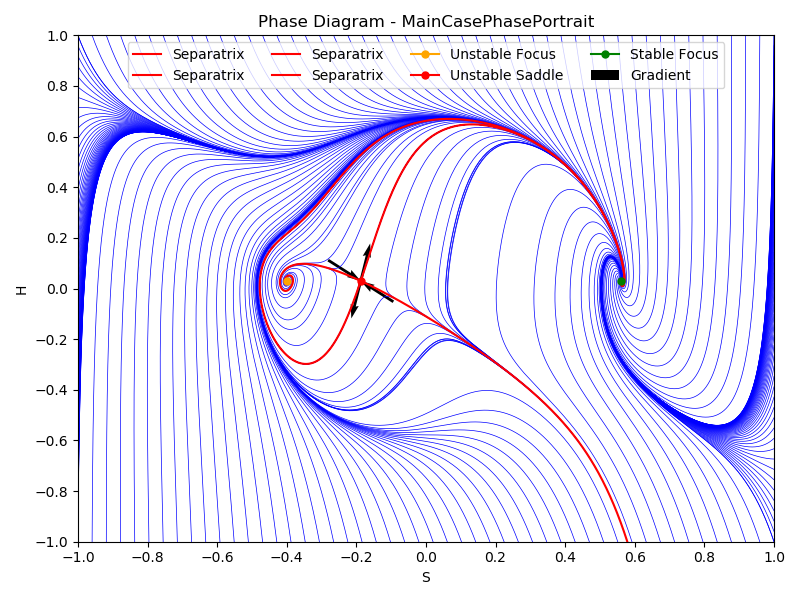
\includegraphics[width=1.0\textwidth]{fig_phaseDiagram.png}
\caption{Phase diagram of the dynamical system of Eqs. \eqref{eq_dyn_system}}
\label{fig_phaseDiagram}
\end{center}
\end{figure}

\section{Endogenous variables}

\subsection{Wages}\label{sec_eq_wage}

\subsection{Interest Rate}\label{sec_eq_interest}

\section{Analysis and open Decisions}
\begin{itemize}
\item Interesting characteristics of recessions: (1) duration, (2) depth of recession (maximum drawdown), (3) speed of recession (time to maximum drawdown), (4) recovery duration (time from maximum drawdown to prior output)
\item Relate these variables to the variance in the exogenous news noise
\item Describe the phase boundaries of the system
\item Determine economically reasonable values for each of the variables e.g. pick the U.S. and do some rough research
\item Robustness: how does the choice in distribution of $\xi_t$ affect the results?
\end{itemize}

\section{Future Work}
\subsection{Current model}
\begin{enumerate}
\item Make technology growth $A_t$ stochastic as well (e.g. Ornstein-Uhlenbeck)
\item Consider policy interventions such as tax/subsidy that would change the savings rate $\kappa$ during recessions
\end{enumerate}

\subsection{Bigger Extensions}
\begin{enumerate}
\item Allow households to dynamically choose how much they save in each period, such as through optimising a utility function. This generates dynamic capital supply.\item Incorporate a stock market / financial system that generates a friction in the credit market, which is another way of making capital supply dynamic. (Gersbach, Rochet \& Sheffel introduced banks into a Solow model). Need to think about introducing a new agent (the banker) or whether to remain in the current setup (households own the firms/stocks so their income depends on it).
\item Allow for a labour market (unemployment) to investigate unemployment effects of recessions and policy options in this regard
\end{enumerate}
\end{document}